\documentclass[11pt]{article}
%\usepackage{fullpage}
\usepackage[top=2cm, bottom=1.5cm, left=1.5cm, right=1.5cm]{geometry}
\usepackage{amsmath,amsthm,amsfonts,amssymb,amscd}
\usepackage{xcolor}
\usepackage{graphicx}
\usepackage[utf8]{inputenc}
\usepackage[english]{babel}
\usepackage{fancyhdr}
\usepackage{wrapfig}

\pagestyle{fancy}
\fancyhf{}
\fancyhead[LO]{Mechanics \& Relativity F3210}
\fancyhead[RO]{Workshop 4: Forces Part 1}
%\fancyfoot[CE,CO]{\leftmark}
%\fancyfoot[LE,RO]{\thepage}

%answers
\usepackage{etoolbox}
\providetoggle{answers}
\settoggle{answers}{false}

\newcommand\vect[1]{\underline{\mathbf{#1}}}
\newcommand\unitvect[1]{\hat{\boldsymbol{#1}}}

\begin{document}

\noindent
\textbf{\textcolor{red}{Please upload your solution to Problem 3 to canvas for marking after the workshop.}}\\
\section*{Problem 1}
A 0.150 kg particle moves along an x axis according to $x(t) = 13.00 + 2.00t + 4.00t^2 - 3.00t^3$, with x in meters and t in seconds. In unit-vector notation, what is the net force acting on the particle at t = 3.40 s?



\section*{Problem 2}
In a laboratory simulation, a standard wood toothpick was shot by pneumatic gun into an oak branch. The toothpick's mass was 0.13~g, its speed before entering the branch was 220 ms$^{-1}$, and its penetration depth was 15~mm. If its speed was decreased at a uniform rate, what was the magnitude of the force of the branch on the toothpick?


\iftoggle{answers}{
\vspace{1cm}
\noindent
SOLUTION:\\

}{}


\noindent

\section*{\textcolor{red}{Problem 3}}
\fbox{\begin{minipage}{\textwidth}
A 200-m-wide river flows due east at a uniform speed of 2.0 ms$^{-1}$. A boat with a speed of 8.0 ms$^{-1}$ relative to the water leaves the south bank pointed in a direction 30$^{\circ}$ west of north. \\
 (a) What is the magnitude of the boat's velocity relative to the ground?\\
 (b) What is the direction of the boat's velocity relative to the ground? \\
 (c) How long does the boat take to cross the river?\\

\end{minipage}}



\section*{Problem 4}


In the figure below, a crate of mass $m = 100$~kg is pushed at constant speed up a frictionless ramp ($\theta= 30.0^{\circ}$ ) by a horizontal force. \\
(a) What is the magnitude of $\vect{F}$?\\
(b) What is the magnitude of the force on the crate from the ramp?
\begin{figure}[h]
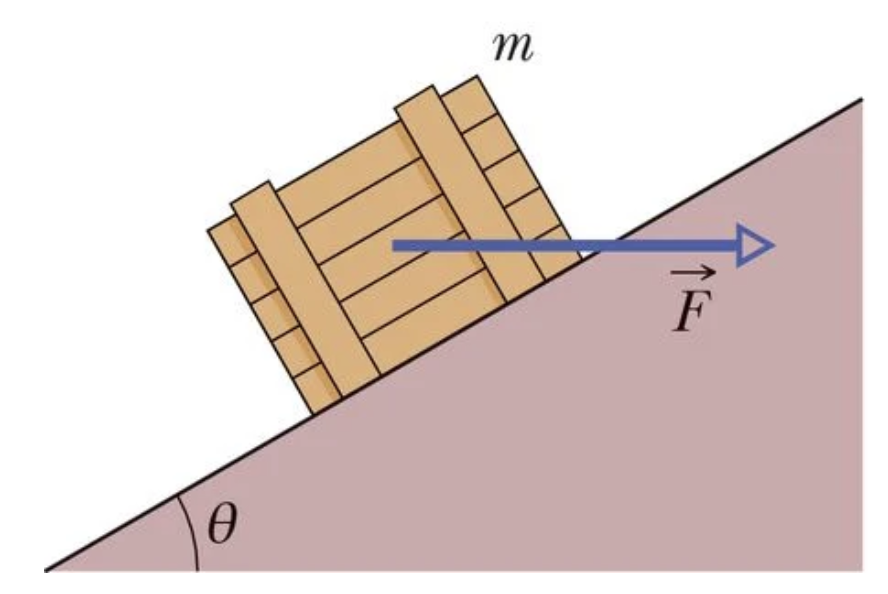
\includegraphics[scale=0.5]{2021-W4-Q4}
\end{figure}


%\vspace{0.5cm}
\section*{Want more practice?}
\small
Further problems on relative motion: Chapter 4.6, 4.7 \\
Further problems on Newton's Laws: Chapter 5.1 \\
Further problems on Forces: Chapter 5.2, 5.3 \\
\end{document}





 




 


